\documentclass[12pt, letterpaper]{article}
\usepackage[margin=1in]{geometry}
\usepackage[utf8]{inputenc}
\usepackage{amsmath}
\usepackage{listings}
\usepackage{graphicx} 
\usepackage{fancyhdr}
\usepackage{booktabs} % For formal tables
\usepackage{float}
\usepackage{hyperref}
\usepackage{indentfirst}
\usepackage{multicol}
\usepackage{bookmark}
\usepackage[T1]{fontenc}
\usepackage{inconsolata}
\usepackage{listings}
\usepackage{color}
\usepackage{xcolor}

\renewcommand{\baselinestretch}{0.9}
\renewcommand{\rmdefault}{ptm}

\pagestyle{fancy}
\fancyhf{}
\setlength{\headheight}{15pt}
\rhead{Nicholas Quandt}
\lhead{McMaster Add-In Iteration 1}
\rfoot{Page \thepage}


\definecolor{bluekeywords}{rgb}{0.13,0.13,1}
\definecolor{greencomments}{rgb}{0,0.5,0}
\definecolor{redstrings}{rgb}{0.9,0,0}
\lstdefinestyle{sharpc}{language=[Sharp]C,
showspaces=false,
showtabs=false,
breaklines=true,
showstringspaces=false,
breakatwhitespace=true,
escapeinside={(*@}{@*)},
commentstyle=\color{greencomments},
keywordstyle=\color{bluekeywords},
stringstyle=\color{redstrings},
basicstyle=\ttfamily,
frame=lr,
rulecolor=\color{blue!80!black}
}

\begin{document}
\begin{titlepage}
   \begin{flushright}
       \vspace*{5cm}
 
       {\Huge \textbf{Design Document}}
 
       \vspace{0.5cm}
        McMaster-Carr Add-In for Autodesk Inventor\\
        Version 1.0.0 $\bullet$ September 30 2019
 
       \vspace{1.5cm}
 
       \textbf{Nicholas Quandt}
       \\
       nicholas.quandt@marquette.edu
       \vfill
       Marquette University Masters Student of\\
       Computational Mathematical and Statistical Sciences\\
       \vspace{1cm}
 
   \end{flushright}
\end{titlepage}

\section{Introduction}
The goal of this project is to create an interface within Autodesk Inventor 2019 that allows for more efficient usage of McMaster Carr's online catalog of 3d Models. 
\section{Languages and Packages}
\begin{multicols}{2}

\begin{itemize}
    \item C\#
    \item XAML
    \item HTML
    \item Autodesk Inventor Interop
    \item CEFSharp v57.0
\end{itemize}
\end{multicols}

\section{Overview of Requirements}
These requirements are a summary of the user stories gathered from the developer and potential users of the add-in.
\begin{enumerate}
\item Runs in Windows 64-bit for Inventor 2019 software.
\item Use Inventor API to add Button for interface.
\item Use McMaster online catalog that has links to 3d models of the majority of their items. Primarily hardware,fasteners etc.
\item Best to keep online interface from McMaster, and somehow open the "form" in inventor to access.
\item Drag and drop from "McMaster interface" into inventor, for either immediate drop into Assembly, or open as individual part.
\item Replace "add to cart" button in HTML with "add to assembly" or "open as part" buttons.
\item Take product information from online catalog and automatically import into Inventor part file.
\item Implement a bill of materials export to send all McMaster items onto clipboard with appropriate QTY per assembly.
\end{enumerate}
\section{Implementation Plan}
McMaster.com is a dynamically generated HTML page that only changes via user exposure to the javascript. A basic HTML scrape of the webpage will not be feasible due to the JS. Thus to gain exposure to the underlying HTML tags needed for properties and file locations, a headless copy of the browser will work to trick the webpage into generating the needed information while the user is interacting with the saving procedure for each part. So far it seems CEFSharp will be the best plan of attack as they offer a headless wrap of google chrome within their package. All processing on the Inventor side of things will be done through the built in .NET API. The browser and add-in will be fully stand alone within Inventor, with no outside installations needed. As is noted in the Notes section, CEFSharp is already built into Inventor 2019, making implementation easier.

\section{User Interface}
\begin{figure}[H]
    \centering
    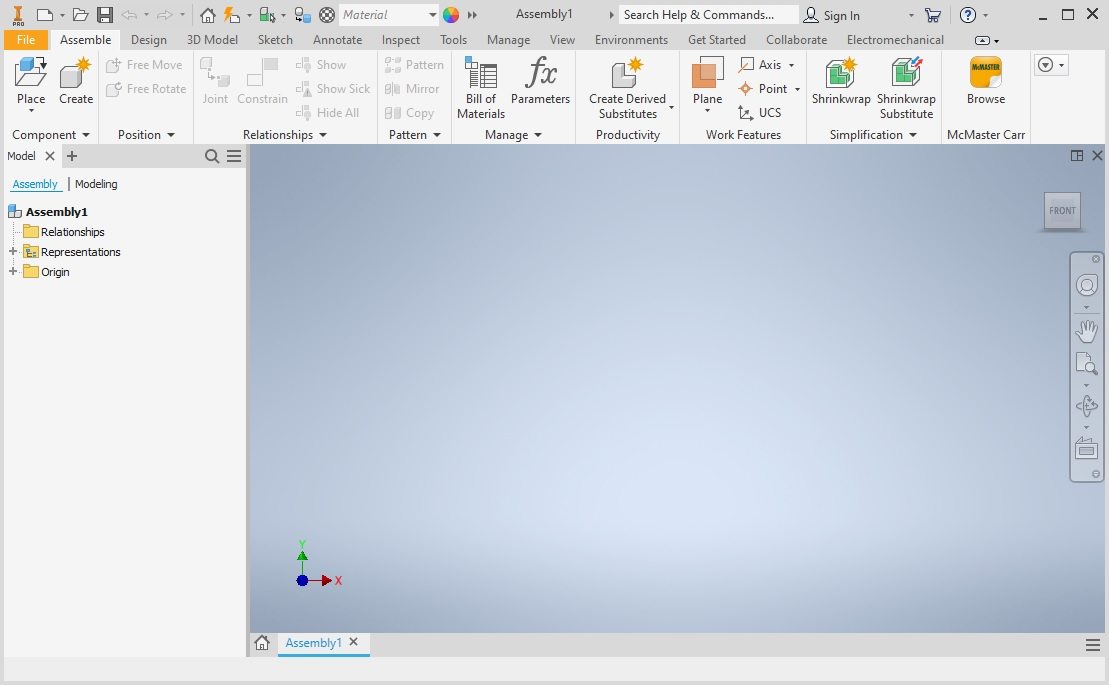
\includegraphics[width=0.5\textwidth]{Figures/mcMasterButton.JPG}
    \caption{The button(far right) addition to the ribbon interface within Autodesk Inventor.}
\end{figure}
\begin{figure}[H]
    \centering
    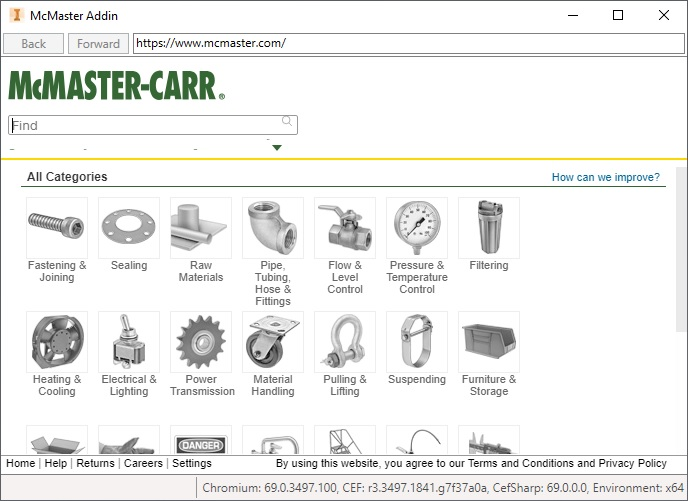
\includegraphics[width=0.5\textwidth]{Figures/webBrowserView.jpg}
    \caption{The browser instance following the button execute event.}
\end{figure}

Iteration 1 allows for the part number to be extracted from the browser form through the mouse hovering link. Iteration 2 aims to take this part number and capture the correct file from the mcmaster database for saving into project.(See Listing 1)\\
\lstset{firstnumber=33,style=sharpc,caption={[Extract1]{Excerpt from MainWindow.xaml.cs}}}
\begin{lstlisting}
currentPartNumber = HoverLinkBehaviour.HoverLink.Substring(urlBase.Length);
System.Diagnostics.Debug.WriteLine(currentPartNumber);
\end{lstlisting}

\newpage
\section{Extra Notes}
\begin{itemize}
    \item CEFSharp v57.0 specifically. v57.0 is built into Inventor 2019, though .WPF package is not, so that needs to be included in release of .dll's.
    \item Possible revisions after all other features:
    \begin{itemize}
        \item Incorporate a "no model" warning for items that do not have corresponding 3d models.
        \item Choose folder to save models per project, or per item.
        \item Always on top.
        \item Comments throughout code for future revising, if ever McMaster online changes.
        \item If final release available, contact McMaster to check usability. 
        \item Solidworks Version??
    \end{itemize}
\end{itemize}
\section{References}

\begin{itemize}
\item https://www.mcmaster.com\cite{McMaster}
\item https://www.autodesk.com/products/inventor/overview
\item https://docs.microsoft.com/en-us/dotnet/
\item https://cefsharp.github.io/
\item https://modthemachine.typepad.com/

\end{itemize}
\begingroup
\renewcommand{\section}[2]{}
\bibliography{srs}
\bibliographystyle{IEEEtran}
\endgroup
\newpage
\section{Appendix A: Story Cards}
\begin{itemize}
    \item [101] As a user I want to be able to use Windows.\\
    Acceptance Criteria: Runs on Windows 64-bit without errors.
    \item [102] As a user I want to use Autodesk Inventor 2019.\\
    Acceptance Criteria: Uses Autodesk Inventor 2019 without errors.
    \item [103] As a user I want to have access to McMaster-Carr catalog from inside of Inventor.\\
    Acceptance Criteria: No outside browser needed to access catalog.
    \item [104] As a user I don't want the interface to change much.\\
    Acceptance Criteria: Uses original online interface.
    \item [105] As a user I should be able to add parts from mcmaster right into my project.
    Acceptance Criteria: No outside program or steps needed to import file.
    \item [106] As a user I would like properties like the material added to my file for me.\\
    Acceptance Criteria: Properties are auto-populated on file addition.
    \item [107] As a developer I would like to use C\# \\
    Acceptance Criteria: All code written with C\# on .NET 4.7.2 or newer
    \item [108] As a developer I shouldn't need to install too many files or packages on the final computer.\\
    Acceptance Criteria: Keep total file count below 3.
    \item [109] As a developer I should well document code to allow for future updates.\\
    Acceptance Criteria: An outside individual can proof read code and follow along without difficulty.
\end{itemize}



\newpage
\section{Appendix B: Code}
StandardAddInServer.cs
\lstset{style=sharpc}
\lstinputlisting{Figures/StandardAddInServer.cs}
\newpage
MainWindow.xaml.cs
\lstinputlisting{Figures/MainWindow.xaml.cs}

\end{document}